\documentclass[twoside]{book}

% Packages required by doxygen
\usepackage{fixltx2e}
\usepackage{calc}
\usepackage{doxygen}
\usepackage[export]{adjustbox} % also loads graphicx
\usepackage{graphicx}
\usepackage[utf8]{inputenc}
\usepackage{makeidx}
\usepackage{multicol}
\usepackage{multirow}
\PassOptionsToPackage{warn}{textcomp}
\usepackage{textcomp}
\usepackage[nointegrals]{wasysym}
\usepackage[table]{xcolor}

% Font selection
\usepackage[T1]{fontenc}
\usepackage[scaled=.90]{helvet}
\usepackage{courier}
\usepackage{amssymb}
\usepackage{sectsty}
\renewcommand{\familydefault}{\sfdefault}
\allsectionsfont{%
  \fontseries{bc}\selectfont%
  \color{darkgray}%
}
\renewcommand{\DoxyLabelFont}{%
  \fontseries{bc}\selectfont%
  \color{darkgray}%
}
\newcommand{\+}{\discretionary{\mbox{\scriptsize$\hookleftarrow$}}{}{}}

% Page & text layout
\usepackage{geometry}
\geometry{%
  a4paper,%
  top=2.5cm,%
  bottom=2.5cm,%
  left=2.5cm,%
  right=2.5cm%
}
\tolerance=750
\hfuzz=15pt
\hbadness=750
\setlength{\emergencystretch}{15pt}
\setlength{\parindent}{0cm}
\setlength{\parskip}{3ex plus 2ex minus 2ex}
\makeatletter
\renewcommand{\paragraph}{%
  \@startsection{paragraph}{4}{0ex}{-1.0ex}{1.0ex}{%
    \normalfont\normalsize\bfseries\SS@parafont%
  }%
}
\renewcommand{\subparagraph}{%
  \@startsection{subparagraph}{5}{0ex}{-1.0ex}{1.0ex}{%
    \normalfont\normalsize\bfseries\SS@subparafont%
  }%
}
\makeatother

% Headers & footers
\usepackage{fancyhdr}
\pagestyle{fancyplain}
\fancyhead[LE]{\fancyplain{}{\bfseries\thepage}}
\fancyhead[CE]{\fancyplain{}{}}
\fancyhead[RE]{\fancyplain{}{\bfseries\leftmark}}
\fancyhead[LO]{\fancyplain{}{\bfseries\rightmark}}
\fancyhead[CO]{\fancyplain{}{}}
\fancyhead[RO]{\fancyplain{}{\bfseries\thepage}}
\fancyfoot[LE]{\fancyplain{}{}}
\fancyfoot[CE]{\fancyplain{}{}}
\fancyfoot[RE]{\fancyplain{}{\bfseries\scriptsize Generated by Doxygen }}
\fancyfoot[LO]{\fancyplain{}{\bfseries\scriptsize Generated by Doxygen }}
\fancyfoot[CO]{\fancyplain{}{}}
\fancyfoot[RO]{\fancyplain{}{}}
\renewcommand{\footrulewidth}{0.4pt}
\renewcommand{\chaptermark}[1]{%
  \markboth{#1}{}%
}
\renewcommand{\sectionmark}[1]{%
  \markright{\thesection\ #1}%
}

% Indices & bibliography
\usepackage{natbib}
\usepackage[titles]{tocloft}
\setcounter{tocdepth}{3}
\setcounter{secnumdepth}{5}
\makeindex

% Hyperlinks (required, but should be loaded last)
\usepackage{ifpdf}
\ifpdf
  \usepackage[pdftex,pagebackref=true]{hyperref}
\else
  \usepackage[ps2pdf,pagebackref=true]{hyperref}
\fi
\hypersetup{%
  colorlinks=true,%
  linkcolor=blue,%
  citecolor=blue,%
  unicode%
}

% Custom commands
\newcommand{\clearemptydoublepage}{%
  \newpage{\pagestyle{empty}\cleardoublepage}%
}

\usepackage{caption}
\captionsetup{labelsep=space,justification=centering,font={bf},singlelinecheck=off,skip=4pt,position=top}

%===== C O N T E N T S =====

\begin{document}

% Titlepage & ToC
\hypersetup{pageanchor=false,
             bookmarksnumbered=true,
             pdfencoding=unicode
            }
\pagenumbering{roman}
\begin{titlepage}
\vspace*{7cm}
\begin{center}%
{\Large My Project }\\
\vspace*{1cm}
{\large Generated by Doxygen 1.8.11}\\
\end{center}
\end{titlepage}
\clearemptydoublepage
\tableofcontents
\clearemptydoublepage
\pagenumbering{arabic}
\hypersetup{pageanchor=true}

%--- Begin generated contents ---
\chapter{Class Index}
\section{Class List}
Here are the classes, structs, unions and interfaces with brief descriptions\+:\begin{DoxyCompactList}
\item\contentsline{section}{\hyperlink{structnode}{node} }{\pageref{structnode}}{}
\item\contentsline{section}{\hyperlink{structnode1}{node1} }{\pageref{structnode1}}{}
\item\contentsline{section}{\hyperlink{structnode__info}{node\+\_\+info} }{\pageref{structnode__info}}{}
\end{DoxyCompactList}

\chapter{File Index}
\section{File List}
Here is a list of all files with brief descriptions\+:\begin{DoxyCompactList}
\item\contentsline{section}{\hyperlink{Lab1_8c}{Lab1.\+c} }{\pageref{Lab1_8c}}{}
\end{DoxyCompactList}

\chapter{Class Documentation}
\hypertarget{structprice}{}\section{price Struct Reference}
\label{structprice}\index{price@{price}}


Collaboration diagram for price\+:
\nopagebreak
\begin{figure}[H]
\begin{center}
\leavevmode
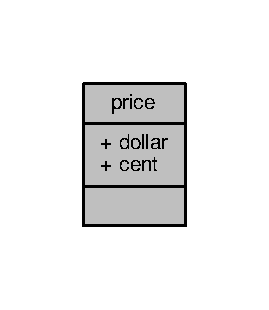
\includegraphics[width=129pt]{structprice__coll__graph}
\end{center}
\end{figure}
\subsection*{Public Attributes}
\begin{DoxyCompactItemize}
\item 
int \hyperlink{structprice_a0e896a2991e2886400502d4f8e5832fc}{dollar}
\item 
int \hyperlink{structprice_a79be97486cb903560bad96132f373907}{cent}
\end{DoxyCompactItemize}


\subsection{Member Data Documentation}
\index{price@{price}!cent@{cent}}
\index{cent@{cent}!price@{price}}
\subsubsection[{\texorpdfstring{cent}{cent}}]{\setlength{\rightskip}{0pt plus 5cm}int price\+::cent}\hypertarget{structprice_a79be97486cb903560bad96132f373907}{}\label{structprice_a79be97486cb903560bad96132f373907}
\index{price@{price}!dollar@{dollar}}
\index{dollar@{dollar}!price@{price}}
\subsubsection[{\texorpdfstring{dollar}{dollar}}]{\setlength{\rightskip}{0pt plus 5cm}int price\+::dollar}\hypertarget{structprice_a0e896a2991e2886400502d4f8e5832fc}{}\label{structprice_a0e896a2991e2886400502d4f8e5832fc}


The documentation for this struct was generated from the following file\+:\begin{DoxyCompactItemize}
\item 
\hyperlink{t_8cpp}{t.\+cpp}\end{DoxyCompactItemize}

\hypertarget{structproduct}{}\section{product Struct Reference}
\label{structproduct}\index{product@{product}}


Collaboration diagram for product\+:
\nopagebreak
\begin{figure}[H]
\begin{center}
\leavevmode
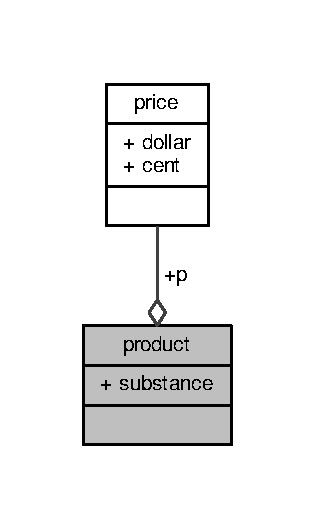
\includegraphics[width=151pt]{structproduct__coll__graph}
\end{center}
\end{figure}
\subsection*{Public Attributes}
\begin{DoxyCompactItemize}
\item 
\hyperlink{structprice}{price} \hyperlink{structproduct_a4987f39c16924c6ef80d5d6055fcc265}{p}
\item 
string \hyperlink{structproduct_a9419ebf0b7d9d0e00ffc4ea9df510fb4}{substance}
\end{DoxyCompactItemize}


\subsection{Member Data Documentation}
\index{product@{product}!p@{p}}
\index{p@{p}!product@{product}}
\subsubsection[{\texorpdfstring{p}{p}}]{\setlength{\rightskip}{0pt plus 5cm}{\bf price} product\+::p}\hypertarget{structproduct_a4987f39c16924c6ef80d5d6055fcc265}{}\label{structproduct_a4987f39c16924c6ef80d5d6055fcc265}
\index{product@{product}!substance@{substance}}
\index{substance@{substance}!product@{product}}
\subsubsection[{\texorpdfstring{substance}{substance}}]{\setlength{\rightskip}{0pt plus 5cm}string product\+::substance}\hypertarget{structproduct_a9419ebf0b7d9d0e00ffc4ea9df510fb4}{}\label{structproduct_a9419ebf0b7d9d0e00ffc4ea9df510fb4}


The documentation for this struct was generated from the following file\+:\begin{DoxyCompactItemize}
\item 
\hyperlink{t_8cpp}{t.\+cpp}\end{DoxyCompactItemize}

\chapter{File Documentation}
\hypertarget{t_8cpp}{}\section{t.\+cpp File Reference}
\label{t_8cpp}\index{t.\+cpp@{t.\+cpp}}
{\ttfamily \#include $<$iostream$>$}\\*
{\ttfamily \#include $<$string$>$}\\*
{\ttfamily \#include $<$vector$>$}\\*
Include dependency graph for t.\+cpp\+:
\nopagebreak
\begin{figure}[H]
\begin{center}
\leavevmode
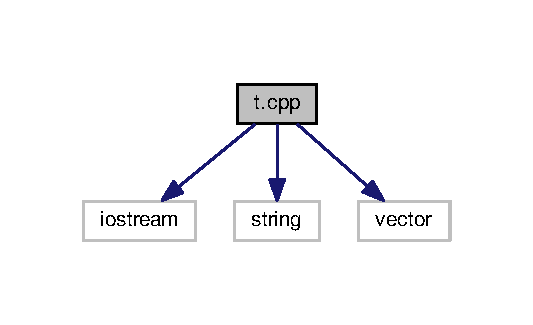
\includegraphics[width=256pt]{t_8cpp__incl}
\end{center}
\end{figure}
\subsection*{Classes}
\begin{DoxyCompactItemize}
\item 
struct \hyperlink{structprice}{price}
\item 
struct \hyperlink{structproduct}{product}
\end{DoxyCompactItemize}
\subsection*{Functions}
\begin{DoxyCompactItemize}
\item 
int \hyperlink{t_8cpp_ae66f6b31b5ad750f1fe042a706a4e3d4}{main} ()
\end{DoxyCompactItemize}


\subsection{Function Documentation}
\index{t.\+cpp@{t.\+cpp}!main@{main}}
\index{main@{main}!t.\+cpp@{t.\+cpp}}
\subsubsection[{\texorpdfstring{main()}{main()}}]{\setlength{\rightskip}{0pt plus 5cm}int main (
\begin{DoxyParamCaption}
{}
\end{DoxyParamCaption}
)}\hypertarget{t_8cpp_ae66f6b31b5ad750f1fe042a706a4e3d4}{}\label{t_8cpp_ae66f6b31b5ad750f1fe042a706a4e3d4}

\begin{DoxyCode}
18 \{
19   vector<string> array[10];
20   array[1].push\_back(\textcolor{stringliteral}{"Hello"});
21   array[1].back().size();
22   \hyperlink{structprice}{price} pr;
23   pr.\hyperlink{structprice_a0e896a2991e2886400502d4f8e5832fc}{dollar} = 3;
24   \hyperlink{structproduct}{product} floss;
25   floss.\hyperlink{structproduct_a4987f39c16924c6ef80d5d6055fcc265}{p} = pr;
26   vector<int> yo[10];
27   yo[2].push\_back(floss.\hyperlink{structproduct_a4987f39c16924c6ef80d5d6055fcc265}{p}.\hyperlink{structprice_a0e896a2991e2886400502d4f8e5832fc}{dollar});
28   yo[3].push\_back(array[1].back().size());
29   yo[4].push\_back(array[1].back().size()+1);
30   \textcolor{keywordflow}{return} 0;
31 \}
\end{DoxyCode}

%--- End generated contents ---

% Index
\backmatter
\newpage
\phantomsection
\clearemptydoublepage
\addcontentsline{toc}{chapter}{Index}
\printindex

\end{document}
